\chapter{Cài đặt công cụ cần thiết}
\label{Chapter1}

\section{Cài đặt Docker}
Để thuận tiện trong việc lập trình và triển khai ứng dụng, hầu hết mọi service trong đề tài đều được thực hiện thông qua Docker.
        \subsection{Tải và cài đặt Docker}
    Truy cập đường dẫn \texttt{https://docs.docker.com/engine/install/}. Tại màn hình này, chọn hệ điều hành như ý (Xem hình ~\ref{fig:docker_download}) và tiến hành tải về, cài đặt Docker với những cấu hình mặc định theo hướng dẫn riêng của từng hệ điều hành.
    \begin{figure}
            \centering
            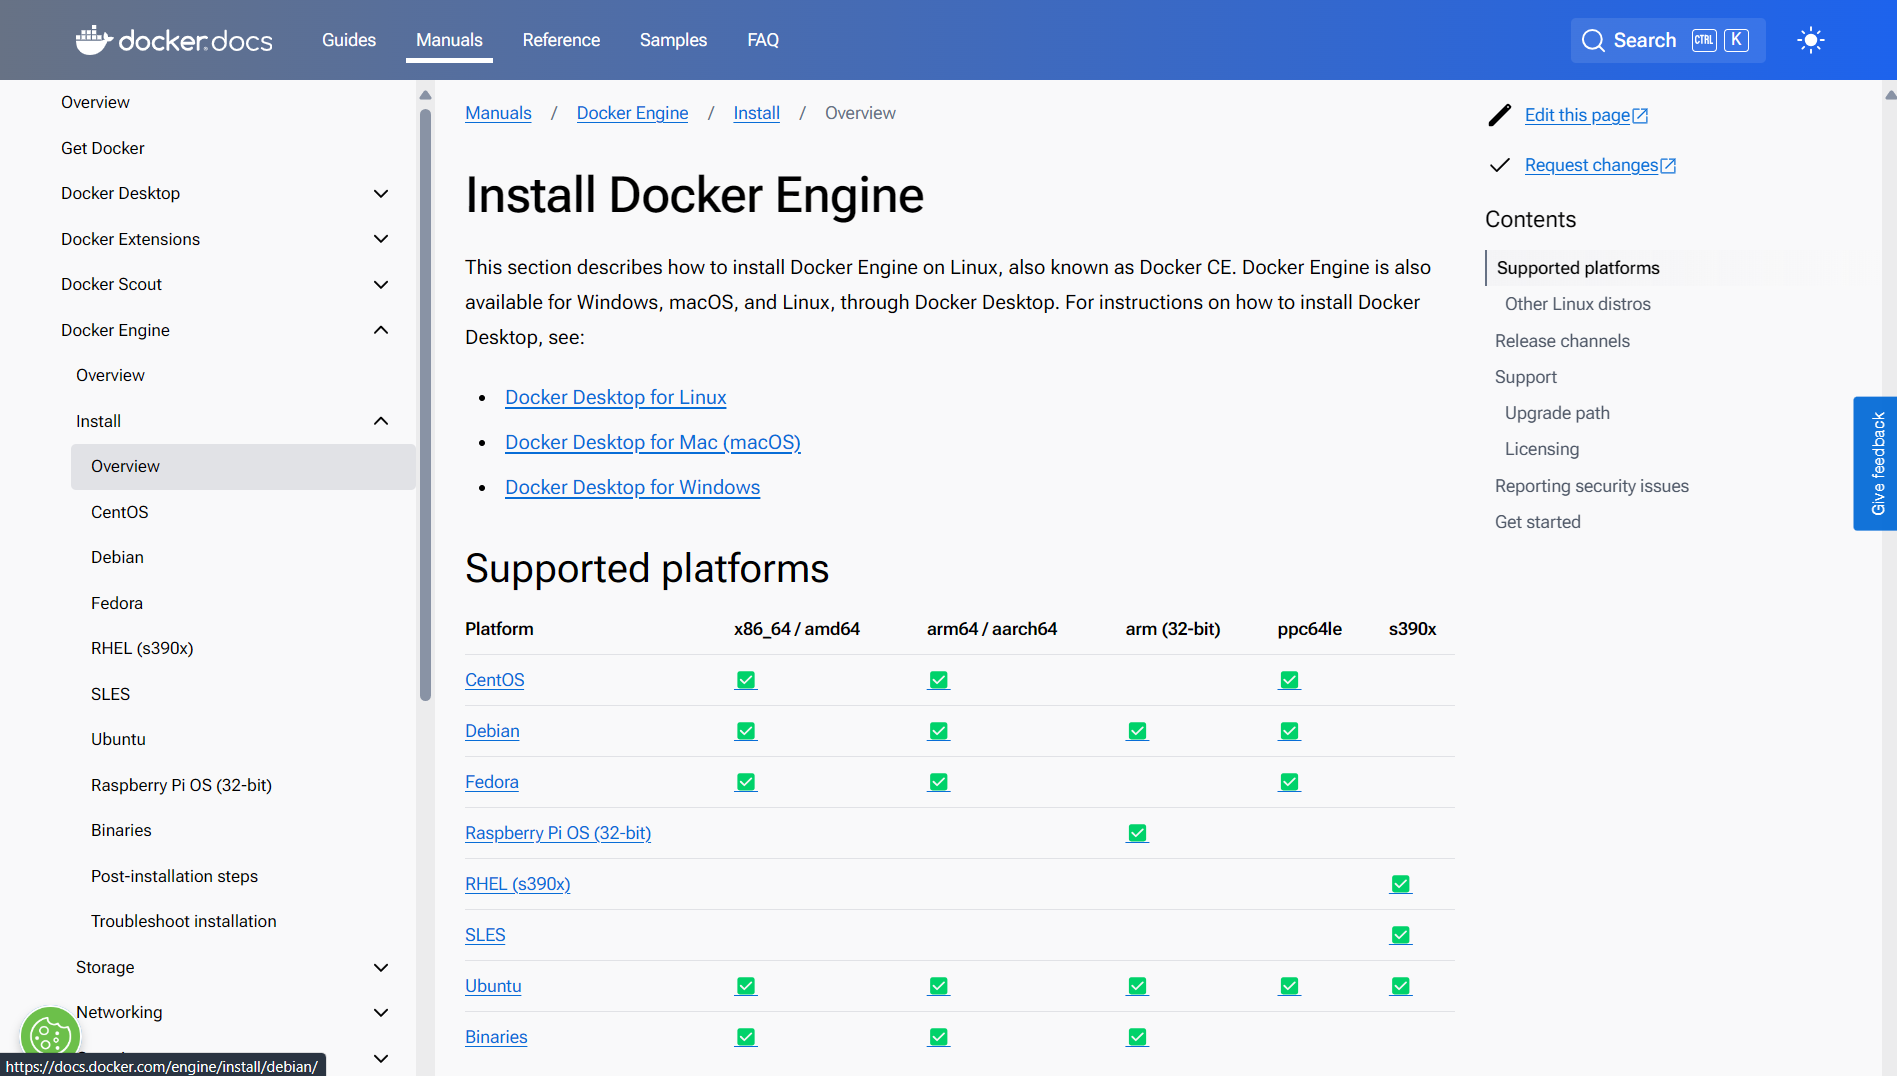
\includegraphics[width=1\linewidth]{docker_download.png}
            \caption{Màn hình chọn hệ điều hành cho Docker}
            \label{fig:docker_download}
    \end{figure}

    \subsection{Tạo tài khoản và đăng nhập DockerHub (không bắt buộc)}
    Sau khi đã cài đặt thành công, ta tiến hành đăng nhập hoặc tạo tài khoản Docker để truy cập Docker Hub.
    \subsection{Kết quả}
    Sau khi đã làm theo hướng dẫn cài đặt trên chủ, Docker sẽ được cài đặt và Docker Engine sẽ được chạy thành công. Để kiểm tra liệu Docker Engine đã được chạy, nhập câu lệnh \texttt{docker ps}.
